\chapter{Design}
\label{ch:design}

This chapter describes the design decisions of the web application and how it supports the project's overall goal.

\section{Technologies}
\label{sec:technologies}
As mentioned in the background section (\ref{sec:plaid}), the web application utilises Plaid for the open banking aspect. It requires a frontend and a backend to follow the authentication flow for ensured security. Most of the tool is written in JavaScript and uses the Next.js framework; however, the backend also features a neural network model written in Python.

\subsection{Next.js}
Next.js is a full-stack React framework by Vercel \cite{Next.js}. It incorporates the React library for the frontend, and supporting API routes for the backend, meaning it is an ideal framework for this project. Other benefits of using Next.js include the ability to perform server-side rendering and intelligent code optimisations.

% \subsubsection{Server-side Rendering}
Server-side rendering (SSR) is when the server computes what files are needed and sends them all in a single response to be displayed instantly. This contrasts with the default client-side rendering (CSR), where a single HTML file is sent to the client. This file may reference JavaScript and CSS files, so the client then downloads these from the server before being able to render the page. The first contentful paint times can be slower for SSR as the server needs to compute what files are needed and send them, whereas for CSR the client can render the HTML only as soon as it is received. However, in CSR the page is not able to be interacted with until the other files are downloaded and executed. Therefore, the total loading time is faster for SSR. In addition, using SSR makes the application's component development less complicated.

% \subsubsection{Automatic Optimisations}
Next.js also has inbuilt automatic optimisations that improve building and serving times. For example, a query to get a user's transactions goes through 3 stages. The first is the initial query from the client to the Next.js API route; then, this accesses the database and queries Plaid's endpoints; finally, Plaid makes the query to the bank, and the response propagates back. Therefore, any optimisations that improve the speed and help avoid slow data loading times are valuable and what Next.js provides by default.

% \subsubsection{Other Benefits}
Next.js is an extremely popular web application meta-framework with over one-hundred-thousand stars on GitHub \cite{NextGitHub}. It is well documented, and there is a large community, so it is easy to find solutions to common problems that may arise. Finally, Next.js is a framework that focuses on the ease of development to maximise productivity, which means the whole experience was more enjoyable and good software engineering practices were followed.

\subsection{TailwindCSS}
As part of the Next.js environment, the website serves JSX components that can be styled as standard HTML elements with CSS. TailwindCSS is a framework that contains a large amount of utility CSS classes. The application incorporates these classes to customise the way the website looks completely.

A different consideration for helping to build the UI is to use a component library. This may have cut down on development time, but they often look generic and unappealing due to the limited ability for customisation. TailwindCSS is more flexible and enables the UI to be built to the exact specification of the design and the developer's vision. Like Next.js, TailwindCSS is also quite popular, with many resources and cheat sheets that aid development. Next.js and TailwindCSS are often used in combination, such as in the t3 web stack, as they synergise well \cite{T3Stack}.

The UI is a big focus for this project, as it is one of the limitations in the current systems that perform similar tasks. The background research found that their interfaces are often ugly and unintuitive. The UI design focuses on being appealing and minimal, so the user has more confidence in the application and, therefore, their finances. Furthermore, the user's data is displayed in an informative and easy-to-understand way, so they are more likely to absorb the information and make better financial decisions.

\subsection{PocketBase}
Part of the authentication flow with Plaid requires that the access tokens are stored to be used later. Each access token can only be associated with one particular user, but a user may have several access tokens. On top of this, a database is needed for basic user authentication where users can sign up and log in. PocketBase was determined to be most appropriate for these use cases due to its simplicity and fast setup.

PocketBase is an ``open source backend consisting of embedded database (SQLite) with real-time subscriptions, built-in auth management, convenient dashboard UI and simple REST-ish API'' \cite{PocketBaseDocs}. It is run as a single executable file, and the Next.js API routes can connect to it locally. In addition, the built-in authentication management enables users to log in and persist their sessions across refreshes, making the user experience much more seamless.

Pocketbase features an interactive UI dashboard for the developer to manage users and aid in bug fixing. This dashboard improves the development experience as it helps to visualise the database structure and manage the tables inside. Finally, PocketBase has a JavaScript SDK that can connect to the database from the API routes. This means that simple JavaScript function calls can be used to interact with the database, rather than complicated REST requests with embedded SQL queries that have more potential for errors.

\subsection{Python and TensorFlow}
Budget prediction was proposed after the research into strategies that help build financial capability. The thought process and reasoning of why a recurrent neural network is used for the budget prediction is explained later (\ref{sec:BudgetPrediction}); but for this section, all that is needed to know that it is implemented in Python, and in particular, using the TensorFlow library.

TensorFlow is a machine learning platform used to help build and optimise many machine learning models. Using this and Python allowed for faster development of the machine learning aspect of the project. Python is a language that is often used for machine learning for a variety of reasons. Nazar Kvartalnyi \cite{PythonML} comments that some of these reasons include the variety of libraries and frameworks, such as TensorFlow, that support the process; that there is an excellent community for giving support during development; and that it is simple, consistent and intuitive. Furthermore, the application developer already has experience with Python and TensorFlow, so there was a lesser learning toll when implementing the budget prediction.

Using Python for the budget prediction does have some drawbacks, such as the added complexity by using a second language, and the extra layer in communication between the application and the neural network. After training the neural network, it is pickled and saved to a file. This file is then loaded and hosted with a Python flask server to be treated like an API. It has a single route that takes the input data and then responds with the neural network's output. This simple solution meant more time was focused on ensuring the neural network is accurate and precise.

\section{UI}
\label{sec:ui}
As mentioned previously, there was a big focus is on making the user interface appealing and intuitive. By working with TailWindCSS, prototype designs could be made in software such as Figma, and then the developer could match the design precisely with appropriate CSS classes and JavaScript functionality.

Despite this, the design process that was instead followed was first to give the components their basic functionality; perform adequate component-based styling; go back to the functionality and modify if appropriate; and finally finish off the styling with the whole page in mind to make sure that is cohesive. This process was more suitable for the project because the styling did not compromise the website's functionality. In addition, on-the-fly styling is an added benefit of TailWindCSS as it allows for quick viewing of designs and fast changes.

\subsection{Authentication Pages}
When a user first visits the site, they must create an account. Research into the limitations of other services showed that having a quick and seamless experience at this stage is vital for the user. This contrasts with applications like Monzo and Revolut, where the signup process is long as they do not only sign up for the analytics but also to make a bank account. The focus for this application is simplicity, so the design for these pages is simple input boxes and a function button to log in or create an account.

\begin{figure}[H]
	\centering
	\includegraphics[width=0.7\textwidth]{images/login_specification.png}
	\caption{Login Page Design}
	\label{fig:LoginPage}
\end{figure}

Above is the basic design for these pages. Most parts are self-explanatory; however, where it says ``(query)'' is where any message or response can be displayed to the user. Examples of these include ``you have successfully logged out'', ``that user does not exist'', or ``incorrect password''; and are given the relevant colours. In addition, the ``don't have an account?'' and ``login'' text are modified appropriately for each page that it is on - for example, if instead, the user is creating an account, it says ``already have an account?'' and ``signup'' respectively.

These pages were the first and only to be styled from a draw.io specification. This is because the process was relatively slow and tedious as it did not maximise the value of using dynamic styling feature of TailwindCSS. The more efficient process outlined in this section's introduction (\ref{sec:ui}) was followed for the remaining of the pages.

\subsection{Dashboard}
Once the minimum strategies for the web application had been determined (transactions, categories, budgets and investments), it was decided that this information would be presented on a single central page, and the ability to switch between the strategies would be done via a header bar. This is so quick access to all the information is possible, but also so that strategies not being viewed are preloaded in the background, avoiding long waits for the information to load and ultimately improving the user experience.

\begin{figure}[H]
	\centering
	
\includegraphics[width=\textwidth]{images/header_navigation_bar.png}
	\caption{Dashboard Navigation Bar}
	\label{fig:DashboardNavigationBar}
\end{figure}

The header bar above (\ref{fig:DashboardNavigationBar}) was the initial design for this dashboard. By default, the transactions strategy is chosen. When hovering over the other strategies, a light-grey bar underneath the strategy name appears; when selected turns this bar orange and removes the bar from the previous strategy. Underneath this bar is the strategy itself; for example, all the recent transactions are below in the transactions strategy.

A limitation in the current systems outlined earlier (\ref{sec:mobile-banking-applications}) is the ability to include several accounts. Furthermore, of the few that do have this feature, none of them have a way to easily enable/disable the incorporation of these accounts in the analytics. This aspect was vital when thinking about the design of the header bar.

On the right of figure \ref{fig:DashboardNavigationBar}, in a slightly different button, there is an accounts dropdown. When clicking on this, all the bank accounts that the current user has linked are displayed here. Each account has a toggle icon to enable/disable the account which can be seen in figure \ref{fig:AccountsDropdown}. Only enabled accounts are included in the analytics, and when switching between strategies, only the selected accounts persist.

An ideal use case for this feature is when a user has several accounts but only wants to see their transactions on their savings accounts. First, they can disable all the other accounts to do so. Then, after getting this analysis, they can quickly re-enable the other accounts when they want to see them all again by just clicking the toggle button.

\section{Strategies}
The only pages in the whole application are the two described above (authentication and dashboard). Each strategy is implemented as a standalone component, and only one at a time is shown on the dashboard. However, as they are all on the same page, they are all styled in a similar way to be cohesive and match the general theme.

\subsection{Transactions}
The transactions strategy is the default strategy shown on the dashboard because it contains the information that is most useful in helping the user can an overview of their finances. By viewing their recent transactions, they can see where money is being spent and where it is coming from, and then make financial adjustments accordingly. Many traditional banks do not allow quick access to this information, and viewing transactions for all the accounts that have been toggled on can be extremely useful in identifying unnecessary expenses.

From Plaid, the endpoint returns a list of transactions in reverse chronological order per account. Each transaction has an account\_id, amount, date, time, location, currency code, merchant name, category (and more) associated with it. The web application groups the transactions from all toggled accounts by their date and then displays each transaction in reverse chronological order.

The transaction is displayed with the merchant name, category, amount and the bank logo of the account it is from. In addition, there is a separate label, for each date above all the transactions for that date. Finally, a distinction between income and expenditure is made by colouring the whole transaction background light-green for income and light-red for expenditure.

\begin{figure}[H]
	\centering
	\includegraphics[width=0.6\textwidth]{images/transaction_labels.png}
	\caption{Example of Reverse Chronological and Date Grouped Transactions}
	\label{fig:TransactionLabels}
\end{figure}

\subsection{Categories}
The categories strategy is also helpful in identifying unnecessary expenses. In this strategy, the application only takes the previous thirty days and also only takes expenditure. It lists all the transactions in reverse chronological order again, but this time they are not grouped by anything. A pie chart is also displayed, where the values are the total amounts for each category. The user can then see the category they spend the most in and the relative amounts. In addition, they can use a filter to show only the expenditure for that category. All this data, again, is only for the toggled accounts.

The difference between this strategy and the transactions strategy is that the transaction strategy emphasises whether the transactions were income or expenditure and to which bank account. In contrast, in the categories strategy, the emphasis is on the categories of the expenditure and the total amount spent in each category. The input data is the same, but it is a different way of presenting it so that the user can get different perspectives on their finances and ultimately make better decisions.

\subsection{Budgets}
Two different methods of performing budget analysis were considered for this strategy. The first method is giving users a budget breakdown based on their income. Following some research, it was found that for the average person, utilising a 50:30:20 budget is highly effective at helping people spend money on necessities while still having money for some treats and putting some aside in savings. The other method is predicting future expenses to incorporate into a user's budget calculations as budget prediction.

\subsubsection{50:30:20 Budget Strategy}

The article \cite{503020Strategy} by N26, a well-respected European bank, explains the strategy in more detail. In essence, it is when a person spends 50\% of their income on needs, spends 30\% of their income on wants, and puts 20\% of their income into savings. Several other articles back up the effectiveness of this strategy and help give it credibility; \cite{503020InCostLivingCrisis} even talks about how this method carries over into the cost of living crisis.

The method does have some disadvantages, however. The major one is that narrowing down which category each expense falls under is challenging. Often people disagree with what is considered essential, so it is already subjective. A typical example, found in several articles, is a gym membership. Some consider it essential, while others put it in 'the wants' section. Other disadvantages include that it is tricky for someone to alter their spending habits, and often if their income is relatively low, it may not even be possible to save 20\% of their income.

The design for this strategy has an input element where the user can enter their income; however, also determining this value from past transactions. The website then breaks down their income into three sections and gives them values for what they can spend on each. For their previous thirty days of transactions, the usual period between each payday, the user can drag and drop each transaction into the three categories to help them see how much they are currently spending. If they spend too much on any, they can adjust accordingly.

\subsubsection{Budget Prediction Strategy}
The other method considered for a budgeting strategy was to perform budget prediction. This involves viewing how much a user has spent in the current month and performing pattern recognition to predict the remaining days. The user can then compare this to a budgeted amount they planned to spend that month and identify if they are on track.

Budget prediction is helpful for people who may, halfway through the month, see that they are under budget and then, for the rest of the month, overspend and exceed their budget. The strategy identifies that they often spend more later on in a month and incorporates it into the prediction. The user can then identify this pattern and account for this so saving money. A different use case is when someone tries to save money for a specific goal. They can see if they are on track to reach their goal by setting a budgeted amount for each month to help adjust their spending habits to reach it.

\subsubsection{Conclusion}
When comparing the two methods, they each have different advantages and disadvantages; however, it is key to consider that the project's main aim is improving financial capability. Therefore, the budget prediction method is more appropriate than the budget breakdown method because it appeals to more users. In addition, it provides analytics that is extremely difficult for the user to replicate themselves, unlike the 50:30:20 method. Also, when predicting future expenses, the user can adjust what they spend sooner before it becomes a problem, thus making it more effective.

\subsection{Investments}
According to Danny's article on Finder.com, a reputable source for financial information and statistics, ``Almost 1 in 5 Brits have owned stocks or shares'' \cite{InvestmentStats}. This is from a survey completed in 2023, which is recent and fact-checked by other journalists from the site. With over 13 million people in Britain alone, adhering to this demographic is valuable and popular. A handy tool, which continues the idea of getting an overview of the user's finances, is a central portfolio manager, where logged-in users can view and track their investments.

This strategy is the only one that does not utilise Plaid to access the data; instead the user adds it themselves. However, it is not a problem as, unlike the other strategies, once the asset has been purchased, they only need to add it once. Following this, when users check their investments, they can see the updated live price and the profit or loss they have made.

In order to perform this strategy, once the user has added their investments, they must be stored. One option is to store them in local storage within the browser. This method is the simplest to implement and, as stored offline, is somewhat secure; however, the disadvantages include that it is only accessible from the same device and browser. Users must add the investments again to access the tool from another device. In addition, if the user clears their browser data, they lose the investment entry, so they must manually add it again.

The other option is to persist the investments using a database. As a PocketBase database is already being used for the application, this only requires a little extra work and complexity. The significant advantages include that, unlike local storage, when using the database, the information is accessible and up to date from any device or browser, so the investment only needs to be added once. Also, by linking the investments to only be accessible by the user who created them, they are incredibly secure and can be treated like the Plaid access tokens.

Ultimately, the database option was chosen because it synergises well with the system's current design and has the same advantages as local storage. The local storage option became the contingency plan, so if during implementation a problem arises, the local storage option can be used.

As well as persisting the investments, the application also gets the current price of the investment to determine if it is profitable. It gets the current price by requesting a service that provides live investment information. Financial modelling prep is an easy-to-use service that provides quick and live stock prices \cite{FMP}, which is ideal for this task. Given the price that the investment was bought for, and the current price, the application can calculate the profit. This information can be displayed as green for positive and red for negative. These colours allow the user to identify which investments are profitable and can continue and which ones are not, so action can be taken.

\section{Budget Prediction}
\label{sec:BudgetPrediction}
Once decided that budget prediction was the method for the budgeting strategy, the actual underlying prediction method was designed. There were three considerations: a basic manual pattern identification method, using linear regression to find the relationship and a neural network to find the trends. Unfortunately, for each of these methods, the only accessible real training data is the author's past three years of transactions. Therefore, this factor was also be considered when deciding which method to use.

\subsection{Manual Pattern Identification}
Manual pattern identification is the simplest and involves manually identifying the patterns. Given the training data, set periods are suggested. The data is split into these, and it is determined which one and by how much is the most significant period. For example, given the three years of transactions, the data is split into the different seasons and it is identified in which season the most is spent. Using this knowledge, the standard prediction value can be increased if a query is requested during this most expensive season.

This method can be repeated on different features, each of different periods, such as weeks, weekends, months, and national holidays. Once many different factors have been analysed, the predictions can be made by combining all of these.

This method is swift at making predictions but is extremely complicated to implement. Furthermore, the predictions may not be very accurate as some features may not be factors, and some features may not have been considered. Ultimately, this method is a trade-off between accuracy for speed and complexity.

\subsection{Linear Regression}
Linear regression is a method for ``modelling the relationship between a scalar response and one or more explanatory variables'' \cite{LinearRegressionWiki}. When applying this to budget prediction, the output expenditure is the scalar response, and the explanatory variables include the budget set out by the user as well as the current date. The model finds the relationship based on the past three years of data, and then, when a query comes in, it can quickly use the learnt relationship to output an expected expenditure.

The main advantage of this method is that it does not involve any manual pattern identification because, instead, the relationship is computed. Despite this, it is still not that accurate as the relationship between expenditure and explanatory variables almost definitely is not linear, which is the major downfall. A solution is to project the input data into a higher dimension. This method allows the model to find a linear relationship in this projected space but becomes a better non-linear relationship in the original space. This solution may improve the accuracy but requires much more computation and may be considered over-engineering for this problem. In addition, it does not even guarantee a better result.

\subsection{Neural Network}
The final option that was considered was to use a neural network. Neural networks take some input data and, with lots of training data, automatically identify the features and learn the relationships. This option has many variations as each model and structure can differ. The neurons themselves can have different activation functions, but also the connections between them. The networks can be feed-forward, with no loops, or be a recurrent neural network, with some feedback (loops). Each layer can have a various number of neurons, and the number of layers can also be varied.

Acknowledging this, provided the network is designed effectively, it can outperform the other two methods in terms of accuracy, which is ideal for this problem. However, the drawbacks include that it involves a lot of testing and tuning to get the best results. The limitation on input data is, therefore, more prevalent.

\subsection{Conclusion}
Out of the three options described above, the most applicable model for the problem of budget prediction is a neural network. This is because it does not rely on manually finding the features to use, so it identifies even the hidden and complex patterns and, after being trained, can generate quick predictions with high accuracy. The implementation of the budget prediction is described in much more detail in section \ref{sec:budgets}, but a quick overall explanation is given below.

Deciding on the neural network's architecture involves lots of trial and error to identify what is most appropriate. Due to its niche nature, there is little academic research on predicting expenditure given past transactions. This meant the problem needed to be generalised. The vital idea that helped was to think of the problem as a time series problem.

The input data can be treated as a time series by modifying it from a list of chronological transactions to the cumulative amount spent each day and resetting every it month. This problem has much more research because time series prediction is a significant area for many industries, such as stock market prediction. Many ideas applied to time series data found that using a recurrent neural network is the most effective.
\section{Software Architecture}

\begin{figure}[H]
	\centering
	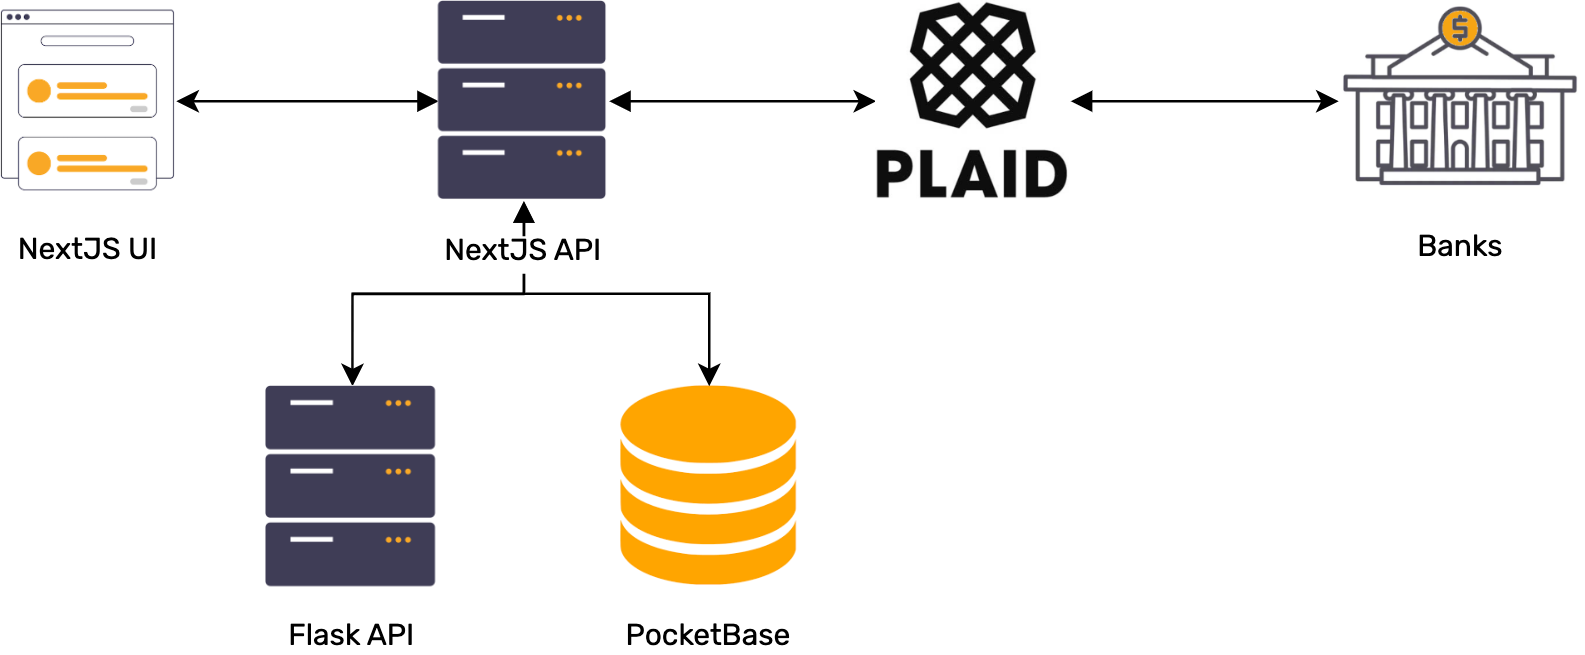
\includegraphics[width=\textwidth]{images/software_architecture.png}
	\caption{Software Architecture}
	\label{fig:SoftwareArchitecture}
\end{figure}

The figure above (\ref{fig:SoftwareArchitecture}) shows the software architecture of the project and the interactions between each service. The four parts on the left have been developed as part of this project, with the two on the right pre-existing entities.

The user interacts with the front end, which is the Next.js UI. Having this separation from the backend is required for the Plaid authentication. The Next.js API routes are how the UI communicates with Plaid and the database. An example API route is ``get\_transactions'', where the backend returns the transactions received from Plaid, which returns the transactions from the bank.

The access tokens and other long-term information, such as the user's login details, are stored in the PocketBase database. Only the backend can access this; furthermore, the access tokens can only be accessed by the user who created them in the first place as an added security measure.

Finally, there is the Python Flask API which contains the budget prediction neural network. This API only has one route. It takes in the input data, propagates it through the neural network, and returns the output. Only the Next.js API routes query it as the input data requires the user's past month's transactions; therefore, they must be requested from Plaid.

When the Budget prediction page is accessed, the frontend queries the Next.js endpoint. The Next.js endpoint first queries Plaid for the transactions, interacts with the database for the access token and then queries the Python Flask API. The Python Flask API returns the prediction to the Next.js API, which returns it to the frontend to be displayed.

\section{Endpoints}
\label{sec:endpoints}
Various Next.js API routes are required for each of the strategies that the web application exhibits. All of these routes are prefixed with ``/api'' to be accessed by the client and all only accept requests using the HTTP POST method. This is because the requests often contain contextual information for the server to decide what to do; for example, they contain the user identifier to determine which user's transactions are being requested.

The information passed between the client and server is in JSON format because it helps represent the data in a structured way, and is easy to parse by both the client and server being written in JavaScript. In addition, Python has a built-in JSON library to work when communicating with the Python Flask API. Also, each route is written such that it can only perform its intended function or return an error. This is because all the error checking is done on the client side to improve security, reduce the amount of code written, and improve the user experience for graceful error handling.

\section{Legal, Ethical and Professional Considerations}
As the application handles sensitive user data, many important considerations were taken to ensure the application is secure and ethical. The most important of these is ensuring that the application only gives financial guidance rather than financial advice.

\subsection{Financial Guidance vs Financial Advice}
In the eyes of the Financial Conduct Authority, financial advice is a ``personalised recommendation'' where the provider is ``responsible and liable for the accuracy, quality and suitability'' \cite{FCA}. On the other hand, financial guidance is a ``suggestion'' or ``service to help you identify your options'', where the provider is still responsible for the accuracy but no longer liable.

In the case of this application, all the information is completely personalised to the user, so the emphasis is made that there are no recommendations. The strategies instead aim to give the user as much information as they want to make financial decisions, rather than making the financial decisions for them. This means each strategy displays information more clearly and practically, rather than taking their information and giving a recommendation.

\subsection{Data Protection}
The correct responsibilities and procedures were followed as part of handling user data. These include the amended Data Protection Act and the General Data Protection Regulation. Despite the application not currently being public facing, the website aims to be eventually, so the application is designed with this in mind. As well as following the strict laws, general data protection techniques are used. For example, the passwords are hashed and salted before being stored in the database, or information specific to a user is only accessible by the creator of that information, not even the developer.

As well as this, there was also an emphasis to try and avoid storing the financial information in the database. In the case of the transactions strategy, some design decisions were adopted to prevent this. For example, rather than storing the recent transactions and only getting the new ones each time, which would have been faster, the application was designed to get all the recent transactions every time as to avoid storing them. Only where necessary, like in the investments strategy, is user-specific financial information stored.